\chapter{Variations of the Uncanny Curve}
In Masahiro Mori’s original hypothesis \cite{original_masahiro}, one can see that if an entity's appearance and movements become indistinguishable from humans, it is possible for the entity to escape the uncanny valley. Moreover, it is even possible that the affinity for an entity, which has overcome the uncanny valley, exceeds the affinity of entities which have not yet fallen into the uncanny valley. If this hypothesis holds, it would have major implications for robotics and other scientific fields as they must strive to design entities whose looks and movements are as similar as possible to that of a human being.\\
On the contrary, it may be possible that the uncanny valley  is not as clearly defined as Masahiro Mori suggests and that it could resemble an uncanny cliff or even an uncanny wall in which the affinity towards entities with perfect or near-perfect human likeness is, in general, lower than that of entities that did not fall into the uncanny valley. In these hypotheses, it may not be advantageous to strive for perfect human likeness.

\section{A Hazy Uncanny Valley}
Masahiro Mori has proposed the uncanny valley as a well-defined graph with a clearly visible dip in affinity as human likeness increases. Furthermore, movement merely steepens the slopes of the uncanny valley in his proposal.
In one of his studies, MacDorman \cite{uncanny_ambiguous} investigated whether the uncanny valley is as clearly defined as Masahiro Mori suggests. To further observe whether human likeness is the main triggering factor, he focused on using androids and robots as stimuli, performing various activities in different environments. For his study, he recruited 56 Indonesian participants, 43 male and 13 female, of whom 13 were 17 to 20 years old, 36 were 21 to 25, 4 were 26 to 30, and 3 were 31 to 35. Having been recruited in an internet cafe and mainly being university students, young professionals, and government workers, the participants had extensive technical experience.\newpage
\begin{wrapfigure}[25]{r}{0.5\textwidth} %this figure will be at the right
    \centering
    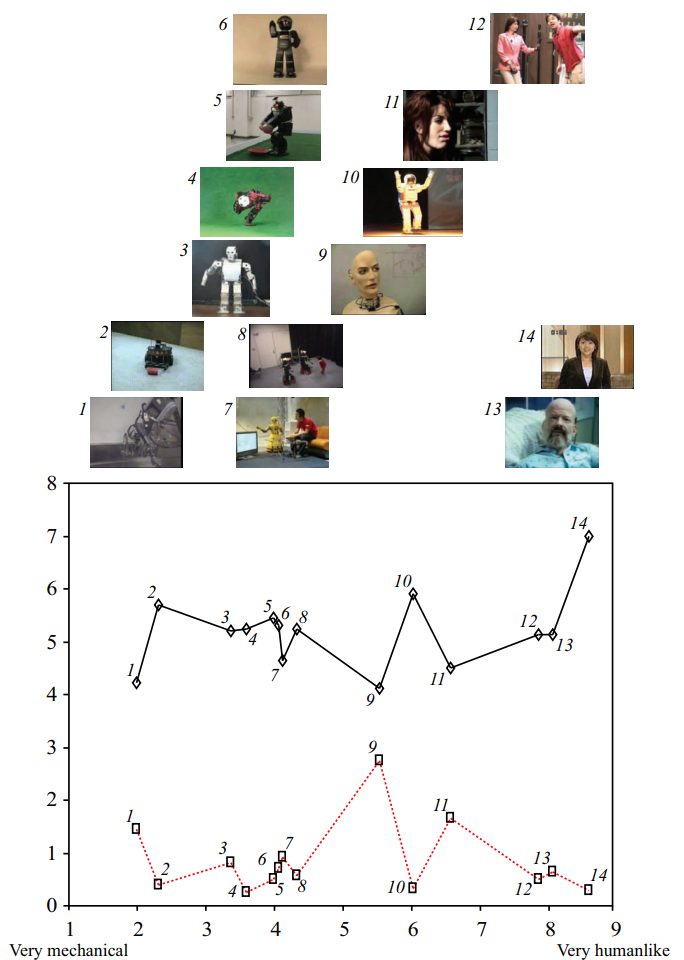
\includegraphics[width=0.5\textwidth]{graphics/hazy_uncanny.png}
    \caption{Result graph of the ratings for the 14 videos.}
    \label{fig:hazyUncanny}
\end{wrapfigure}
The study procedure consisted of a questionnaire in which the participants had to rate 14 video clips, which were 30 to 60 seconds in length, on a nine-point mechanical versus human-like scale, a nine-point strange versus familiar scale, and a
ten-point eeriness scale. The main focus was placed on the selected videos, which consisted of a mobile robot (Pioneer II), a manipulator arm, seven humanoid robots (Rovovie-M3, HR-2, VisiON Nexta, Chronio, Robovie, Wakamaru, Asimo), two android heads (K-bot, Eva), two androids (Philip K. Dick, Repliee Q1Expo), and one human being. The entities depicted in the videos performed different actions in different contexts, sometimes also with speech accompaniment.\\
Figure \ref{fig:hazyUncanny} shows the videos used together with the evaluations of the questionnaire. The solid line plots the relationship between perceived human likeness and perceived familiarity. The dashed line plots the relationship between
perceived human likeness and eeriness. The results of his study show that there is not one particular, uncanny valley for a particular range of human likeness. Therefore, the study  concludes that human likeness is only one of many factors influencing the extent of the uncanny valley effect.\\
From this study, one can conclude that in the real world scenarios with many different influences and situations in which one might encounter the uncanny valley,  it may not only be triggered by the appearance of an entity alone but by many different influences in the respective situation. This creates a much more difficult picture of the uncanny valley than Masahiro Mori suggested. However, the question of whether it is possible to overcome the uncanny valley remains open in this study.

\section{An Uncanny Cliff}
A study by Bartneck et al. \cite{uncanny_cliff} tried to plot the uncanny valley, emphasising the last ascending section of the curve. Furthermore, the referred study also dealt with the question of whether highly human-like androids are perceived as more likeable when they are being framed as robots.\\
In this study, a framing and an anthropomorphism experiment were conducted. Framing contained three conditions: human, robot and none. Anthropomorphism consisted of four conditions real human, manipulated human, computer graphic and android. Additionally, only in the robot framing condition, two additional anthropomorphisms were present: humanoid and pet robot. For the experiment, only pictures of entities that either exist or are highly similar to existing entities were chosen. 
With a questionnaire, the human likeness and the likeability of the stimuli were measured.
To ensure the framing conditions of this study, three different questionnaires with different framings of the pictures were created. The pictures were either framed as human, robot or only as a face for a neutral comparison in each different framing. For each anthropomorphism category, three different pictures were shown to the participants. 
58 people participated in the study aged between 18 and 41 years. 28 of which were female, and 30 were male.
Each of the 18 chosen stimuli was presented to the participants twice. Once with a question about the liking towards the entity, which could be rated on a scale from one to seven and once with 7-point semantic differential scales consisting of the values fake/natural, machinelike/human-like, unconscious/conscious, artificial/lifelike, nice/awful, friendly/unfriendly, kind/unkind, and pleasant/unpleasant. This resulted in 36 questions that the participants had to answer on a computer in a randomised order.\\
This study concluded that the framing of the entities had no significant influence on the measurements. The pictures were evaluated independently from whether they were labelled as human, robot or face, and the labelling did not impact the likeability or human likeness in a negative or positive way.
 However, the questionnaire results showed that anthropomorphism had a significant influence on human likeness and likeability. The participants most liked the pictures of toy robots and humanoids. Even though a slight upwards trend in likability towards highly human-like entities was noted, not even the pictures of humans reached the affection level of the pictures of toy robots. Based on these results, the study speculates that even the most human-like androids are not liked as much as toy robots or humanoids. Therefore the study suggests a revised graph of Mori's original graph where there may be small valleys, but the main feature is a cliff which is depicted in figure \ref{fig:uncannyCliff}.
\begin{wrapfigure}[13]{r}{0.5\textwidth} %this figure will be at the right
    \centering
    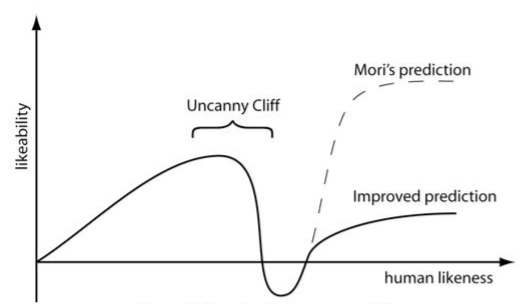
\includegraphics[width=0.5\textwidth]{graphics/uncanny_cliff.png}
    \caption{Hypothesised uncanny cliff.}
    \label{fig:uncannyCliff}
\end{wrapfigure}
In summary, figure \ref{fig:uncannyCliff} would, therefore, not describe an uncanny valley but an uncanny cliff.
The results of this study would imply that it is unwise to attempt to build highly human-like entities since a machinelike robot would be liked more. However, the study mentions that to test the hypothesis further, more studies need to be conducted with participants from different cultures, as the group of participants in the presented study consisted only of Japanese people, who are stereotypically thought of as being more avid robot-aficionados than other cultures.

\section{An Uncanny Wall}
Both in robotics and the creation of virtual characters for films and other media, ever-improving technology is allowing progress to be made towards increasing realism. Based on these improvements, Angela Tinwell and Mark Grimshaw \cite{uncanny_wall} designed a study to examine and plot the curve of the uncanny valley by using videos of virtual characters.\\
For the study, Tinwell et al. chose 100 participants, 92 of them were males and eight females, mainly university students from the creative technology field and professionals working within this academic sector and the video game industry. The selected focus group for the study consisted exclusively of people with much knowledge about informatics and game design and art and, therefore, a lot of exposure and comprehension of the uncanny valley. Furthermore, significantly more men were selected for the study and no information was given about their age.\\%TODO   
\begin{wrapfigure}[16]{r}{0.6\textwidth} %this figure will be at the right
    \centering
    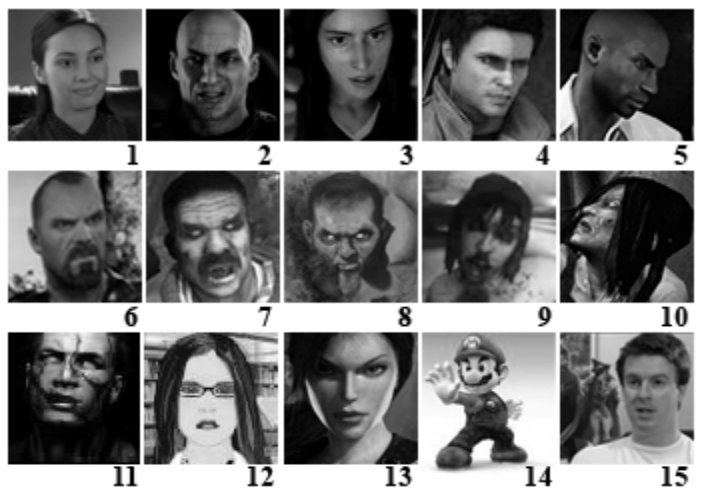
\includegraphics[width=0.6\textwidth]{graphics/uncanny_wall.png}
    \caption{The 15 characters chosen for the study.}
    \label{fig:uncannyWall}
\end{wrapfigure}
The method of the study consisted of a web-based questionnaire in which the participants had to rate 14 video clips of a selection of virtual characters and one video clip of a real human, which were placed in different settings and engaged in different activities, on a nine-point scale how human-like they perceived the characters and how strange or familiar they perceived the character. The video clips were made up of six photorealistic characters, five zombie characters, a photorealistic human-like zombie, three stylised human-like characters and one real human, as seen in figure \ref{fig:uncannyWall}\\
The study results show that the real person was found to be the most familiar and the most human-like by the participants. The six photorealistic characters were found to be very familiar and very human-like, but they could not achieve the ratings of the real person. All zombie-like characters reached shallow familiarity and low human likeness. 
The three stylised human-like characters had received very different ratings. For example, Mario from Mario and Sonic at the Olympic Games was rated as very familiar but not very human-like, and Lara Croft from Lara Croft Tomb Raider: The Action Adventure was rated as very familiar but only in the higher midfield of human likeness. 
\newpage
\begin{wrapfigure}[17]{r}{0.5\textwidth} %this figure will be at the right
    \centering
    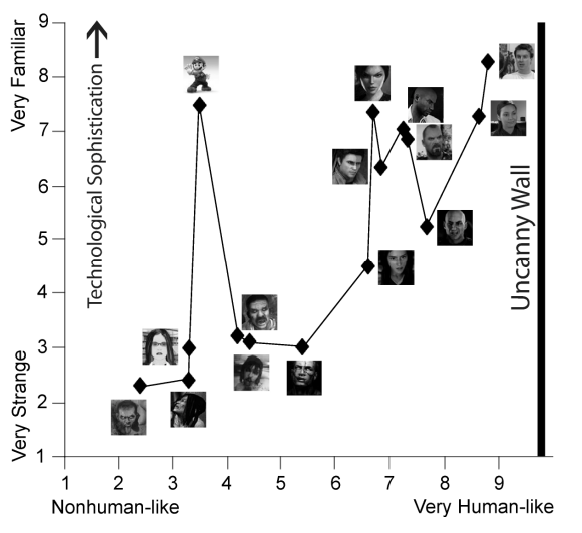
\includegraphics[width=0.5\textwidth]{graphics/uncanny_wall_graph.png}
    \caption{Hypothesized uncanny wall.}
    \label{fig:uncannyWallGraph}
\end{wrapfigure}
As seen from the constructed graph \ref{fig:uncannyWallGraph}, no single valley is found.
Therefore, it can be assumed that the uncanny valley lacks the clarity proposed by Masahiro Mori and paints a more complex picture with multiple influences affecting the familiarity with human-like entities felt by participants.  The fact that no virtual character could outperform a real person, even though all participants were previously exposed to the effects of the uncanny valley in their everyday lives, suggests that an uncanny wall can better define the uncanny valley. Therefore it may be impossible to traverse the uncanny valley defined by Masahiro Mori. Furthermore, the study assumes that with the factor of time, audiences do not get used to the uncanny valley effect, but that time leads to an increasing discernment on the part of viewers to more small details which do not perfectly resemble real humans. Through this sophistication of discernment, the uncanny wall rises with time.\\
This study thus paints a new picture of the uncanny valley, which is impossible to overcome, even with ever-improving technological possibilities. However, it is also worth mentioning that the study's statements should be again validated by conducting the study again with the new possibilities in the development of human-like designs which have emerged in recent times. In such a repeated study, more participants who are not all familiar with the subject matter should be chosen. Finally, when selecting the characters, care should be taken that they are not known to the participants to not influence their ratings.







